\documentclass{standalone}
\usepackage{tikz}
\usepackage{amsmath}
\usetikzlibrary{calc, tikzmark, shapes, shapes.arrows, arrows, positioning}
\usetikzlibrary{decorations.fractals,%
decorations.shapes,%
decorations.text,%
decorations.pathmorphing,%
decorations.pathreplacing,%
decorations.footprints,%
decorations.markings}

\newcommand{\mat}[1]{\boldsymbol{\mathrm{#1}}}

\begin{document}
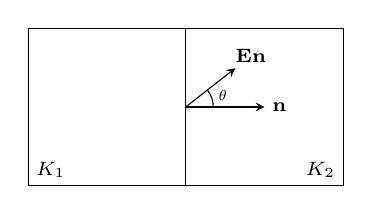
\begin{tikzpicture}
	\scriptsize
	\def\angle{38}
	\def\rad{.8}
	\draw (0,0) grid[step=2] (4,2); 
	\draw[->, >=stealth] (2,1) -- (3,1) node[right] {$\mat{n}$}; 
	\draw[->, >=stealth] (2,1) -- +(\angle:\rad) node[shift={(\angle:.25cm)}] {$\mat{E}\mat{n}$}; 
	\draw (2.35,1) arc(0:38:.35) node[right,pos=.64] {\scalebox{.75}{$\theta$}}; 
	\node[anchor=south west] at (0,0) {$K_1$}; 
	\node[anchor=south east] at (4,0) {$K_2$}; 

	% --- projection onto normal and tangential --- 
	% \draw[densely dashed, opacity=.25] (2,{1+\rad*sin(\angle)}) -- ({2+\rad*cos(\angle)}, {1+\rad*sin(38)}); 
	% \draw[densely dashed, opacity=.25] ({2+\rad*cos(\angle)}, 1) -- ({2+\rad*cos(\angle)}, {1+\rad*sin(38)}); 
	% \draw[decorate,decoration={brace,amplitude=1pt}, xshift=-.5mm] (2,1) -- (2,{1+\rad*sin(\angle)}) node[midway,xshift=-1.5mm] {\scalebox{.5}{$\beta$}}; 
	% \draw[decorate,decoration={brace,amplitude=1pt}, yshift=-.5mm] ({2+\rad*cos(\angle)},1) -- (2,1) node[midway,yshift=-1.5mm] {\scalebox{.5}{$\alpha$}}; 
\end{tikzpicture}
\end{document}